\label{sec:4.3}

%%%%%%%%%%%%%%%%%%%%%%%%%%%%%%%%%%%%%%%%%%%%%%%%%%%%%%%
% Dynamic Linearity
%%%%%%%%%%%%%%%%%%%%%%%%%%%%%%%%%%%%%%%%%%%%%%%%%%%%%%%

The dynamic performance of an ADC is determined by the effective number of bits (ENOB). Figure~\ref{fig:coldadc_fft} shows the Fast-Fourier Transform (FFT) from one of the ADC channels.  The ENOB across ADC channels at LN$_2$ temperature is generally fairly uniform with a mean value of 10.6 bits and a spread of about 0.3 bits. 
\begin{figure}[htb]
\centering
%\begin{minipage}[b]{1.0\textwidth}
\begin{center}
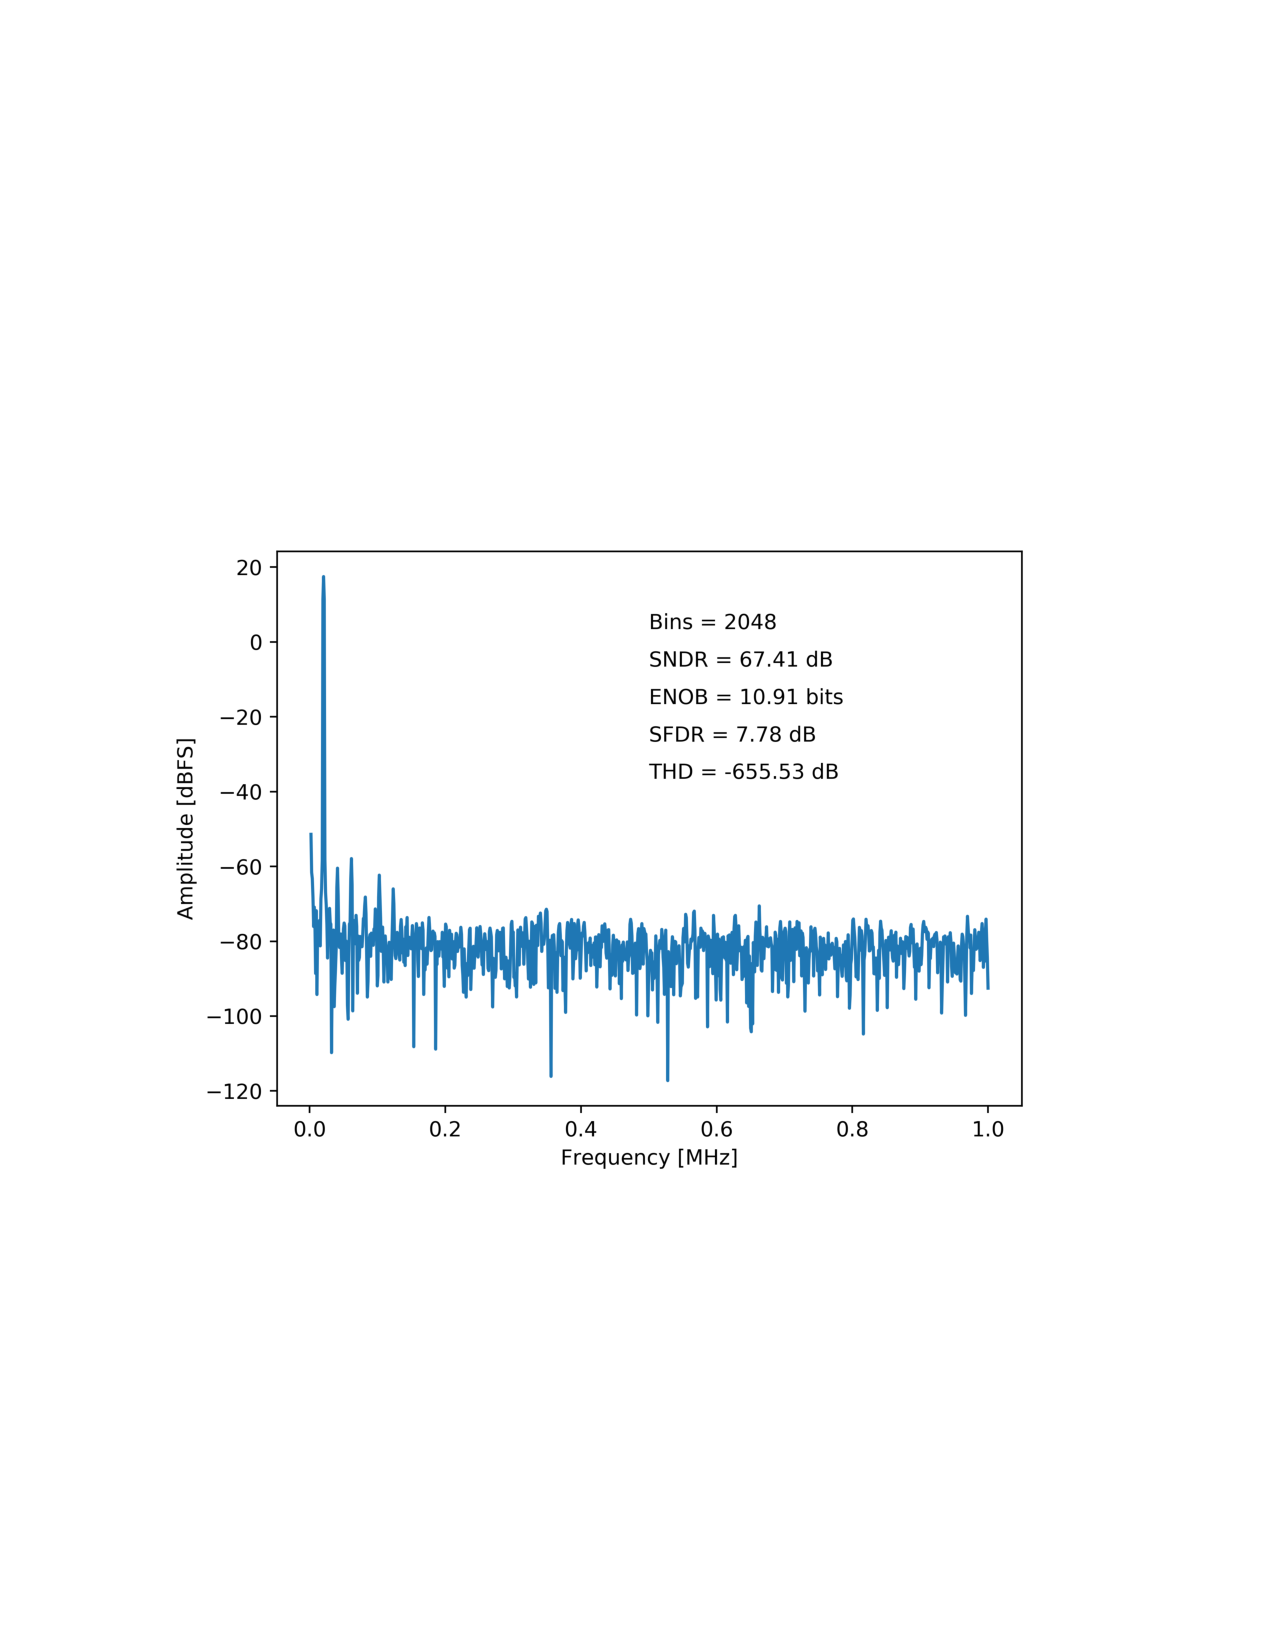
\includegraphics[width=0.7\textwidth]{figures/fft_Sinusoid_20KHz_SE-SHA-ADC0_NomVREFPN_2M_v1.pdf}
\end{center}
%\end{minipage}
\caption{FFT.}
\label{fig:coldadc_fft}
\end{figure}



